%%%%%%%%%%%%%%%%%%%%%%%%%%%%%%%%%%%%%%%%%%%%%%%%%%%%%%%%%%%%%%%%%%%%
% Authors: A. Herrera, M. Morales, M. Ruíz
% Tittle: Tryton
% 							 DDSI 2017
%%%%%%%%%%%%%%%%%%%%%%%%%%%%%%%%%%%%%%%%%%%%%%%%%%%%%%%%%%%%%%%%%%%%

%!TEX root = ../tryton.tex
%!TEX language = es

\section{Instalación}

    \subsection{Descarga}

	\begin{frame}[fragile=singleslide]{Descarga}

        \fontsize{10}{8}\selectfont

        \begin{itemize}
            \item \textbf{Dependencias:} \texttt{python3-lxml} y todo su árbol de dependencias.
        \end{itemize}

        \begin{mycode}[bash]
sudo apt-get build-dep python3-lxml
sudo apt-get install python3-lxml
		\end{mycode}

        \begin{itemize}
            \item Descarga con \textbf{pip} - Pip install Python
            \item \textbf{pip} viene por defecto en cualquier distribución de Python.
        \end{itemize}

        \begin{mycode}[bash]
# Actualizar pip
sudo pip install -U pip
sudo pip install trytond
sudo pip install tryton-client
        \end{mycode}
        \begin{tikzpicture}[remember picture,overlay]
        \node at (9,1.7) {
\includegraphics[width=0.15\textwidth]{./Images/danger.png}};
        \node at (9,0.8) {Ubuntu 16.04 LTS};
        \end{tikzpicture}

    \end{frame}

    \subsection{Uso}

	\begin{frame}[fragile=singleslide]{¿Cómo utilizar tryton?}
        \begin{itemize}
            \item Configuración y ejecución del servidor - {\color{ChetwodeBlue}\textbf{trytond}}.
            \item Bases de datos disponibles: \textbf{PostgreSQL}, SQLite, MySQL. (Gracias a \texttt{python-sql}).
            \item Acceso al servidor desde el cliente - {\color{ChetwodeBlue}\textbf{tryton-client}}.
            \item Demo
        \end{itemize}
        \begin{center}
            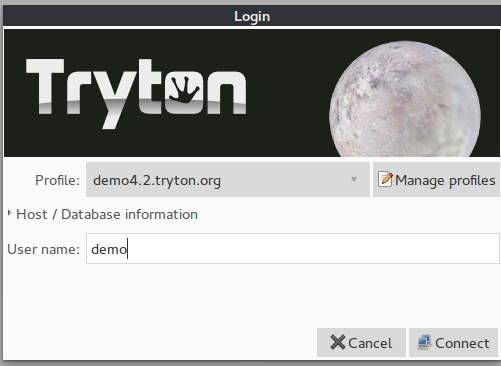
\includegraphics[width=0.55\textwidth]{./Images/demo.png}
        \end{center}
	\end{frame}

    \begin{frame}[fragile=singleslide]{¿Cómo utilizar tryton?}
        \vspace*{-0.3cm}
        \begin{columns}
            \column{0.6\textwidth}
            \begin{center}
                {\color{ChetwodeBlue}Tryton client}
            \end{center}
            \vspace*{-0.1cm}
            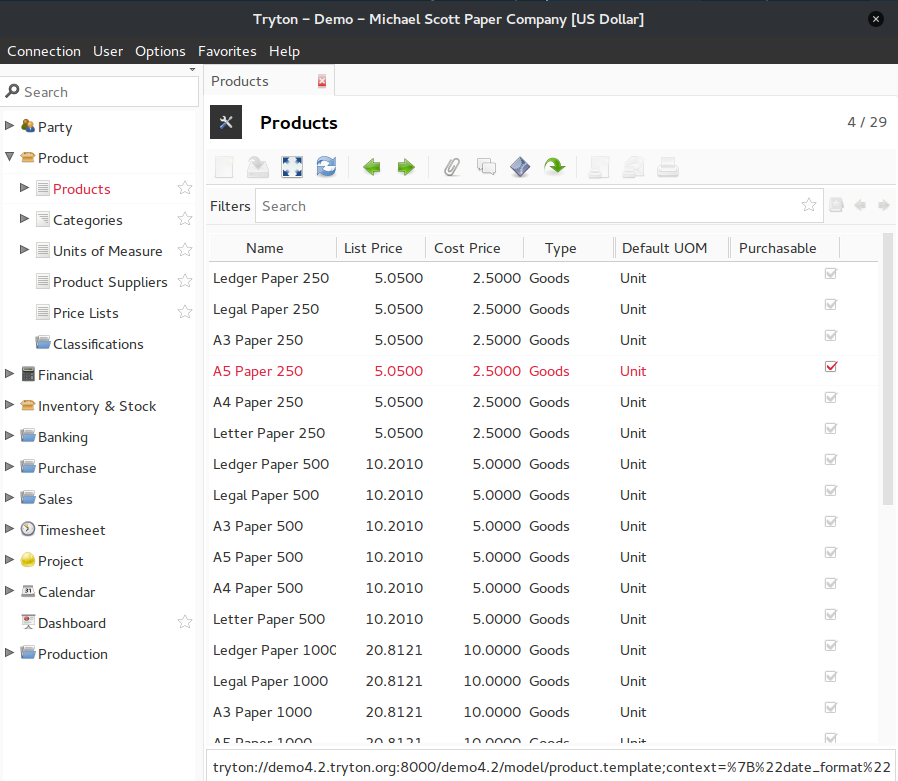
\includegraphics[width=\textwidth]{./Images/demo-products.png}
            \column{0.5\textwidth}
            \begin{center}
                {\color{ChetwodeBlue}Sao web interface}
            \end{center}
            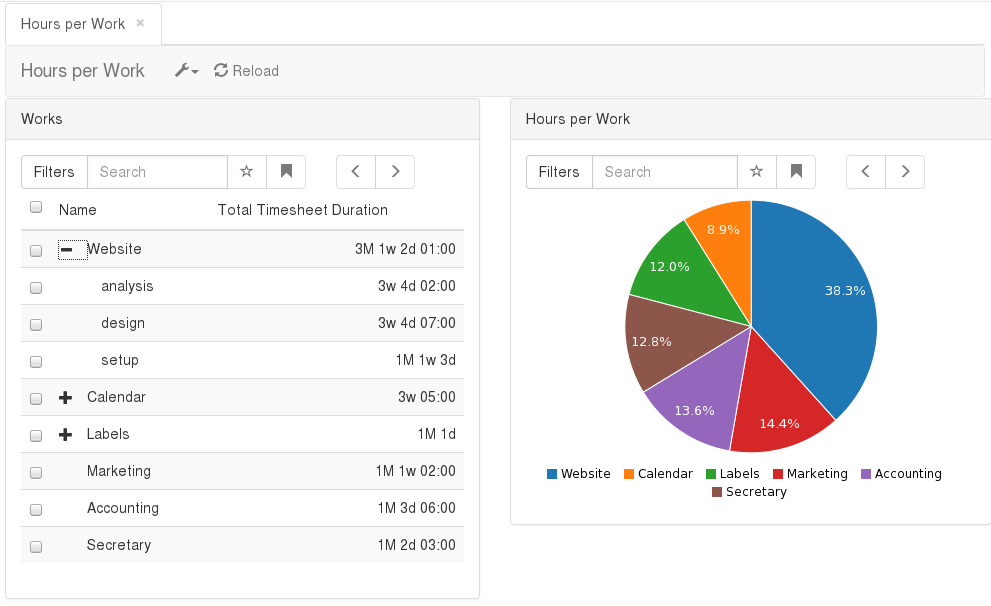
\includegraphics[width=\textwidth]{./Images/tryton-sao.png}
        \end{columns}

        \begin{center}
            {\color{TurkishRose}\textbf{Interfaz amigable}}
        \end{center}
	\end{frame}

%	\begin{frame}[fragile=singleslide]{Configuración de la base de datos}
%
%		\begin{mycode}[bash]
%sudo apt install sqlite3
%#creates an sqlite DB in the current folder you are in
%sqlite3 tryton_db.sqlite ""
%
%#initializes the DB
%#you will be prompted for the DB admin password. Choose one.
%trytond-admin -c /home/erp/trytond.conf -d /home/erp/tryton_db --all
%		\end{mycode}
%	\end{frame}
